\documentclass[12pt]{article}
\usepackage{graphicx}
\begin{document}
{\bf Names:} Jack Bracewell, Milan Misak, Craig Ellis\\
{\bf Usernames:} jb2910, mm5510, ce710 \\
{\bf Group Number: 28}  \\

{\bf Assignment 2:} Decision Trees Algorithm \\ \\

{\bf Implementation details} \\
\begin{itemize}
  \item Cross-validation was done by first generating a cell array of the binary targets for each emotion. Then, inside a for-loop, each fold is removed from the set of examples in turn, leaving a set used to train the decision tree, and the fold used to test the resulting trees for accuracy. A running total is kept of correct answers, along with a confusion matrix updated on each loop. These are used to define how well the decision trees performed.
  \item Best attributes were selected by ...
  \item Average results were computed by ...
\end{itemize}
Include at least: cross-validation, best attribute selection, computing average results\\

{\bf Generated trees} \\
\begin{figure}[h]
  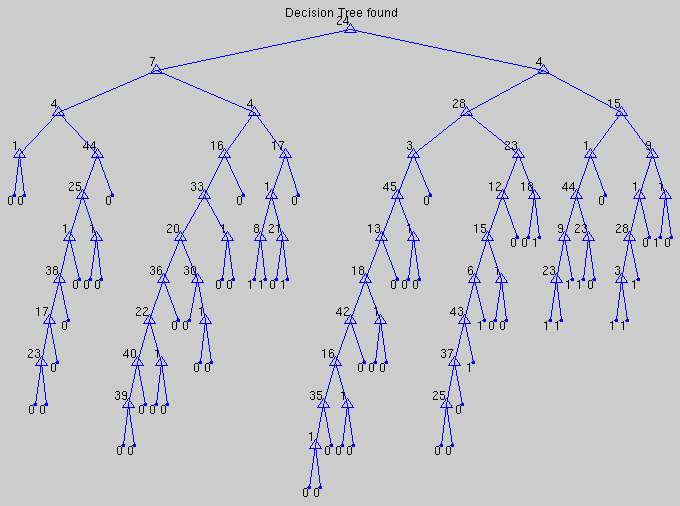
\includegraphics{report-images/tree1.png}
  \caption{Tree for emotion 1}
\hfill
  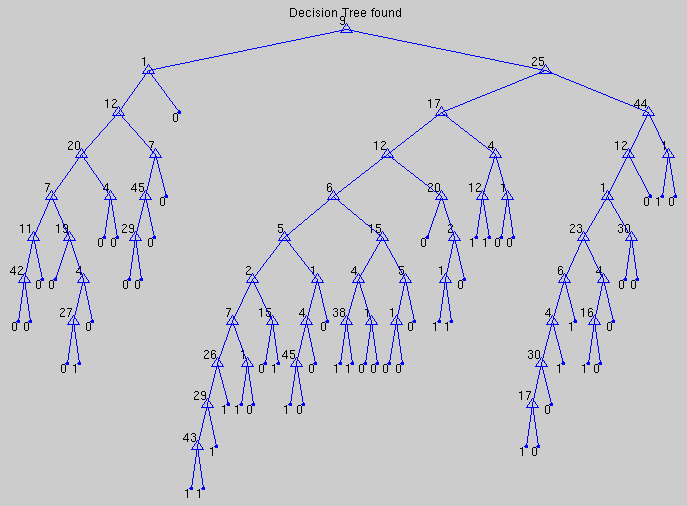
\includegraphics{report-images/tree2.png}
  \caption{Tree for emotion 2}
\hfill
  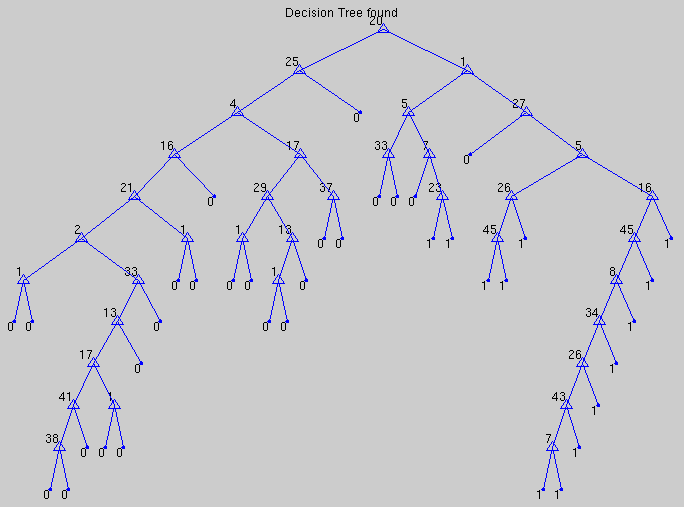
\includegraphics{report-images/tree3.png}
  \caption{Tree for emotion 3}
\hfill
  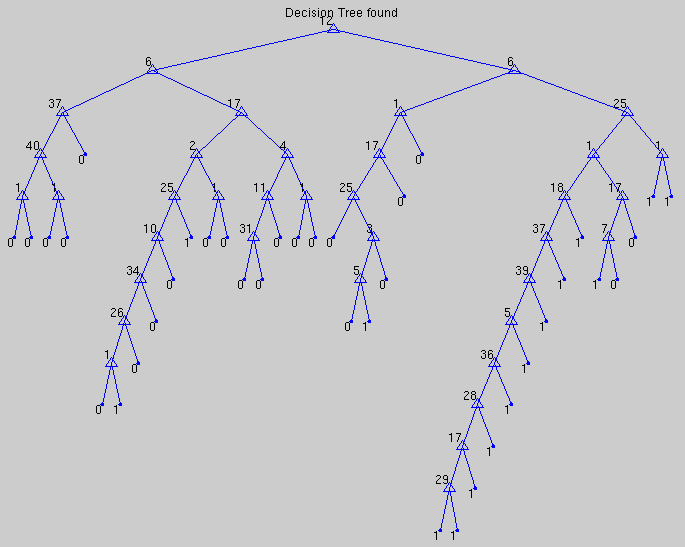
\includegraphics{report-images/tree4.png}
  \caption{Tree for emotion 4}
\hfill
  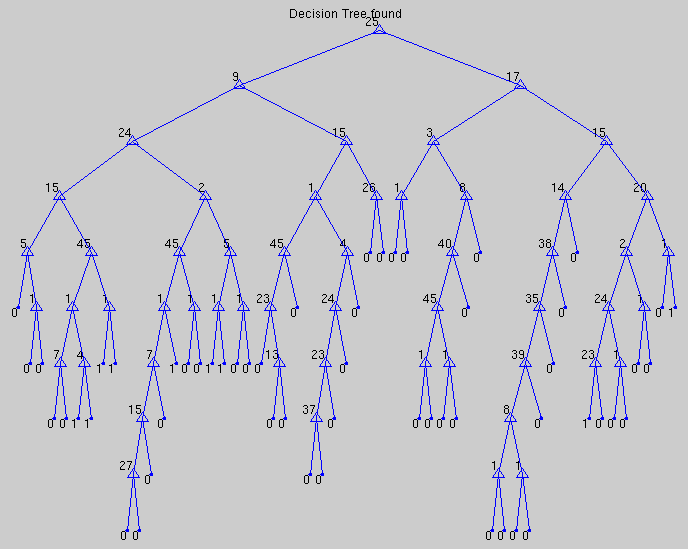
\includegraphics{report-images/tree5.png}
  \caption{Tree for emotion 5}
\hfill
  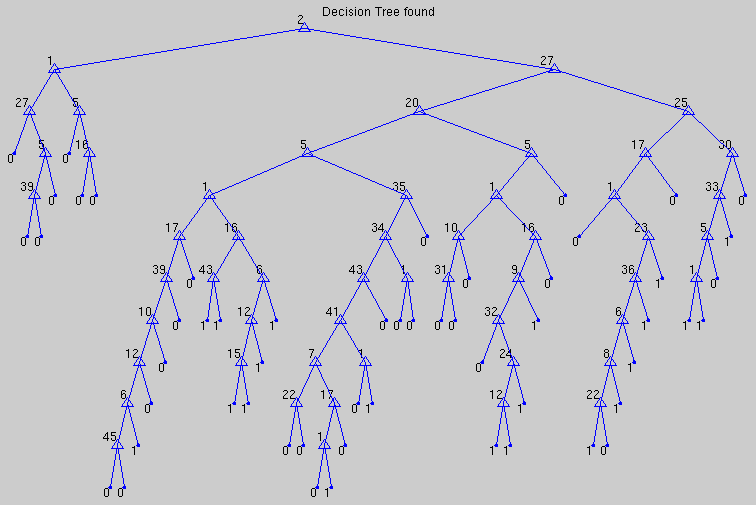
\includegraphics{report-images/tree6.png}
  \caption{Tree for emotion 6}
\end{figure}
Just diagrams \\

{\bf Evaluation results} \\
Confusion matrix, av. classification rate, av. precision/recall rates, F-measure; include comments \\

{\bf Ambiguity} \\
Answer sheet question \\

{\bf Pruning} \\
Answer sheet question\\

{\bf Code Flowchart} \\
Flowchart of code workings\\

\end{document}
